\documentclass[]{book}
\usepackage{lmodern}
\usepackage{amssymb,amsmath}
\usepackage{ifxetex,ifluatex}
\usepackage{fixltx2e} % provides \textsubscript
\ifnum 0\ifxetex 1\fi\ifluatex 1\fi=0 % if pdftex
  \usepackage[T1]{fontenc}
  \usepackage[utf8]{inputenc}
\else % if luatex or xelatex
  \ifxetex
    \usepackage{mathspec}
  \else
    \usepackage{fontspec}
  \fi
  \defaultfontfeatures{Ligatures=TeX,Scale=MatchLowercase}
\fi
% use upquote if available, for straight quotes in verbatim environments
\IfFileExists{upquote.sty}{\usepackage{upquote}}{}
% use microtype if available
\IfFileExists{microtype.sty}{%
\usepackage{microtype}
\UseMicrotypeSet[protrusion]{basicmath} % disable protrusion for tt fonts
}{}
\usepackage[margin=1in]{geometry}
\usepackage{hyperref}
\hypersetup{unicode=true,
            pdftitle={Estatística, Ciência de Dados e Sociedade},
            pdfauthor={Steven Dutt Ross \& Alexandre Silva},
            pdfborder={0 0 0},
            breaklinks=true}
\urlstyle{same}  % don't use monospace font for urls
\usepackage{natbib}
\bibliographystyle{apalike}
\usepackage{color}
\usepackage{fancyvrb}
\newcommand{\VerbBar}{|}
\newcommand{\VERB}{\Verb[commandchars=\\\{\}]}
\DefineVerbatimEnvironment{Highlighting}{Verbatim}{commandchars=\\\{\}}
% Add ',fontsize=\small' for more characters per line
\usepackage{framed}
\definecolor{shadecolor}{RGB}{248,248,248}
\newenvironment{Shaded}{\begin{snugshade}}{\end{snugshade}}
\newcommand{\KeywordTok}[1]{\textcolor[rgb]{0.13,0.29,0.53}{\textbf{#1}}}
\newcommand{\DataTypeTok}[1]{\textcolor[rgb]{0.13,0.29,0.53}{#1}}
\newcommand{\DecValTok}[1]{\textcolor[rgb]{0.00,0.00,0.81}{#1}}
\newcommand{\BaseNTok}[1]{\textcolor[rgb]{0.00,0.00,0.81}{#1}}
\newcommand{\FloatTok}[1]{\textcolor[rgb]{0.00,0.00,0.81}{#1}}
\newcommand{\ConstantTok}[1]{\textcolor[rgb]{0.00,0.00,0.00}{#1}}
\newcommand{\CharTok}[1]{\textcolor[rgb]{0.31,0.60,0.02}{#1}}
\newcommand{\SpecialCharTok}[1]{\textcolor[rgb]{0.00,0.00,0.00}{#1}}
\newcommand{\StringTok}[1]{\textcolor[rgb]{0.31,0.60,0.02}{#1}}
\newcommand{\VerbatimStringTok}[1]{\textcolor[rgb]{0.31,0.60,0.02}{#1}}
\newcommand{\SpecialStringTok}[1]{\textcolor[rgb]{0.31,0.60,0.02}{#1}}
\newcommand{\ImportTok}[1]{#1}
\newcommand{\CommentTok}[1]{\textcolor[rgb]{0.56,0.35,0.01}{\textit{#1}}}
\newcommand{\DocumentationTok}[1]{\textcolor[rgb]{0.56,0.35,0.01}{\textbf{\textit{#1}}}}
\newcommand{\AnnotationTok}[1]{\textcolor[rgb]{0.56,0.35,0.01}{\textbf{\textit{#1}}}}
\newcommand{\CommentVarTok}[1]{\textcolor[rgb]{0.56,0.35,0.01}{\textbf{\textit{#1}}}}
\newcommand{\OtherTok}[1]{\textcolor[rgb]{0.56,0.35,0.01}{#1}}
\newcommand{\FunctionTok}[1]{\textcolor[rgb]{0.00,0.00,0.00}{#1}}
\newcommand{\VariableTok}[1]{\textcolor[rgb]{0.00,0.00,0.00}{#1}}
\newcommand{\ControlFlowTok}[1]{\textcolor[rgb]{0.13,0.29,0.53}{\textbf{#1}}}
\newcommand{\OperatorTok}[1]{\textcolor[rgb]{0.81,0.36,0.00}{\textbf{#1}}}
\newcommand{\BuiltInTok}[1]{#1}
\newcommand{\ExtensionTok}[1]{#1}
\newcommand{\PreprocessorTok}[1]{\textcolor[rgb]{0.56,0.35,0.01}{\textit{#1}}}
\newcommand{\AttributeTok}[1]{\textcolor[rgb]{0.77,0.63,0.00}{#1}}
\newcommand{\RegionMarkerTok}[1]{#1}
\newcommand{\InformationTok}[1]{\textcolor[rgb]{0.56,0.35,0.01}{\textbf{\textit{#1}}}}
\newcommand{\WarningTok}[1]{\textcolor[rgb]{0.56,0.35,0.01}{\textbf{\textit{#1}}}}
\newcommand{\AlertTok}[1]{\textcolor[rgb]{0.94,0.16,0.16}{#1}}
\newcommand{\ErrorTok}[1]{\textcolor[rgb]{0.64,0.00,0.00}{\textbf{#1}}}
\newcommand{\NormalTok}[1]{#1}
\usepackage{longtable,booktabs}
\usepackage{graphicx,grffile}
\makeatletter
\def\maxwidth{\ifdim\Gin@nat@width>\linewidth\linewidth\else\Gin@nat@width\fi}
\def\maxheight{\ifdim\Gin@nat@height>\textheight\textheight\else\Gin@nat@height\fi}
\makeatother
% Scale images if necessary, so that they will not overflow the page
% margins by default, and it is still possible to overwrite the defaults
% using explicit options in \includegraphics[width, height, ...]{}
\setkeys{Gin}{width=\maxwidth,height=\maxheight,keepaspectratio}
\IfFileExists{parskip.sty}{%
\usepackage{parskip}
}{% else
\setlength{\parindent}{0pt}
\setlength{\parskip}{6pt plus 2pt minus 1pt}
}
\setlength{\emergencystretch}{3em}  % prevent overfull lines
\providecommand{\tightlist}{%
  \setlength{\itemsep}{0pt}\setlength{\parskip}{0pt}}
\setcounter{secnumdepth}{5}
% Redefines (sub)paragraphs to behave more like sections
\ifx\paragraph\undefined\else
\let\oldparagraph\paragraph
\renewcommand{\paragraph}[1]{\oldparagraph{#1}\mbox{}}
\fi
\ifx\subparagraph\undefined\else
\let\oldsubparagraph\subparagraph
\renewcommand{\subparagraph}[1]{\oldsubparagraph{#1}\mbox{}}
\fi

%%% Use protect on footnotes to avoid problems with footnotes in titles
\let\rmarkdownfootnote\footnote%
\def\footnote{\protect\rmarkdownfootnote}

%%% Change title format to be more compact
\usepackage{titling}

% Create subtitle command for use in maketitle
\newcommand{\subtitle}[1]{
  \posttitle{
    \begin{center}\large#1\end{center}
    }
}

\setlength{\droptitle}{-2em}
  \title{Estatística, Ciência de Dados e Sociedade}
  \pretitle{\vspace{\droptitle}\centering\huge}
  \posttitle{\par}
  \author{Steven Dutt Ross \& Alexandre Silva}
  \preauthor{\centering\large\emph}
  \postauthor{\par}
  \predate{\centering\large\emph}
  \postdate{\par}
  \date{2017-08-20}

\usepackage{booktabs}
\usepackage{amsthm}
\makeatletter
\def\thm@space@setup{%
  \thm@preskip=8pt plus 2pt minus 4pt
  \thm@postskip=\thm@preskip
}
\makeatother

\usepackage{amsthm}
\newtheorem{theorem}{Teorema}[chapter]
\newtheorem{lemma}{Lemma}[chapter]
\theoremstyle{definition}
\newtheorem{definition}{Definição}[chapter]
\newtheorem{corollary}{Corollary}[chapter]
\newtheorem{proposition}{Proposição}[chapter]
\theoremstyle{definition}
\newtheorem{example}{Example}[chapter]
\theoremstyle{definition}
\newtheorem{exercise}{Exercise}[chapter]
\theoremstyle{remark}
\newtheorem*{remark}{Remark}
\newtheorem*{solution}{Solution}
\begin{document}
\maketitle

{
\setcounter{tocdepth}{1}
\tableofcontents
}
\chapter{Introdução}\label{introducao}

sei lá\ldots{}. podemos escrever um monte de coisas de introdução
aqui\ldots{}. o que vc acha?

\chapter{Inferência Estatística}\label{inferencia-estatistica}

Texto baseado no livro \emph{A Estatística Básica e sua Prática}
\citet{Moore}

Ao extrair uma amostra, sabemos exatamente todas as respostas dos
entrevistados. Entretanto, não queremos somente isso. Queremos também
construir conclusões sobre a população. Em outras palavras, queremos
\textbf{generalizar os resultados da amostra para a população}. O
processo para isso é chamado inferência estatística. De fato, o nosso
unico interesse em uma amostra aleatória é que ela forneça informação
que possa ser generalizada para a população maior.

A média da amostra \textbf{não} será exatamente igual à méda da
população (evento muito raro. chance mínima disso acontecer). Se
pudessemos extrair uma \textbf{outra amostra da mesma população}, os
resultados dessa nova amostra poderia nos conduzir a conclusões
diferentes. Como ter certeza que as conclusões baseadas em uma única
amostra estão corretas? A inferencia estatística usa a linguagem da
\textbf{probabilidade} para expressar o grau de confibilidade de nosas
conclusões.

Assim, esperamos que a amostra forneça alguma informação sobre a média
populacional, embora saibamos que não será livre de erros. isso pode ser
representado como uma equação:

\[\bar{X}=\mu+\epsilon\]

Onde \(\bar{X}\) é a média amostral, \(\mu\) (a letra grega \emph{mi}) é
a média populacional e \(\epsilon\) é o erro amostral. Esse ultimo termo
dfa equação pode assumir valores positivos e negativos (erro para mais
ou para menos). O que essa equação está querendo dizer é:

Estatística Amostral = Parametro Populacional + Erro Amostral

As duas abordagens mais comuns da inferência estatística para isso são
chamadas de:

\begin{enumerate}
\def\labelenumi{\arabic{enumi}.}
\tightlist
\item
  Intervalos de confiança
\item
  Teste de Hipóteses
\end{enumerate}

Ambos os tipos de inferência baseiam-se nas distribuições amostrais de
estatísticas.

\section{Distribuições Amostrais}\label{distribuicoes-amostrais}

Suponha que na cidade do Rio de Janeiro só temos cinco empresas, isto é,
uma população de 5 unidades. Vamos imaginar que os lucros dessas
empresas foram de 8, 9, 10, 11 e 12 unidades monetárias. É facil
verificar que o parâmetro da população da média é igual a 10 unidades.
Vamos representar esse parâmetro por uma letra grega. Em outras
palavras, vamos considerar \[\mu=10\]. Além disso, o desvio padrão
desses valores é \[ \sigma=1,41\].

\begin{Shaded}
\begin{Highlighting}[]
\NormalTok{empresa<-}\KeywordTok{c}\NormalTok{(}\DecValTok{8}\NormalTok{,}\DecValTok{9}\NormalTok{,}\DecValTok{10}\NormalTok{,}\DecValTok{11}\NormalTok{,}\DecValTok{12}\NormalTok{)}
\KeywordTok{mean}\NormalTok{(empresa)}
\end{Highlighting}
\end{Shaded}

\begin{verbatim}
## [1] 10
\end{verbatim}

Dessa população-alvo de 05 elementos, quero extrair todas as possíveis
amostras de 03 elementos, com reposição, conforme mostrado na tabela ao
lado.

\begin{table}

\caption{\label{tab:DA2}Amostras de tamanho 3 e Média dessas amostras}
\centering
\begin{tabular}[t]{lr}
\toprule
Amostra\_Extraida\_tamanho\_3 & Media\_Amostra\\
\midrule
8,8,8 & 8.00\\
8,8,9 & 8.33\\
8,8,10 & 8.67\\
8,8,11 & 9.00\\
8,8,12 & 9.33\\
\addlinespace
8,9,8 & 8.33\\
8,9,9 & 8.67\\
8,9,10 & 9.00\\
8,9,11 & 9.33\\
8,9,12 & 9.67\\
Etc & NA\\
\bottomrule
\end{tabular}
\end{table}

Nessa tabela extraimos (com reposição) todas as amostras possíveis. A
primeira amostra foi aquela onde sorteamos o lucro. a segunda amostra
foi 8,8,9. Na segunda coluna temos a média dessas amostras sorteadas.

Interessante notar que a média da amostra igual a 8 é muito rara e só
acontece uma unica vez. Isso só ocorre quando a amostra é igual a 8,8,8.
Já a média da amostra igual a 8,33 ocorre em três situações:

\begin{enumerate}
\def\labelenumi{\arabic{enumi}.}
\tightlist
\item
  8,8,9
\item
  8,9,8
\item
  9,8,8
\end{enumerate}

Após calculado o valor de média é possível agrupar de acordo com o
número de vezes que esses valores aparecem.

Nessas três situação a resultante será a média 8,33. Fazendo a
frequência de todas as médias possíveis encontramos a seguinte tabela:

\begin{table}

\caption{\label{tab:DA3}Média da amostras e Frequência dessas médias}
\centering
\begin{tabular}[t]{rr}
\toprule
Media & Frequencia\\
\midrule
8.00 & 1\\
8.33 & 3\\
8.67 & 6\\
9.00 & 10\\
9.33 & 15\\
\addlinespace
9.67 & 18\\
10.00 & 19\\
10.33 & 18\\
10.67 & 15\\
11.00 & 10\\
\addlinespace
11.33 & 6\\
11.67 & 3\\
12.00 & 1\\
\bottomrule
\end{tabular}
\end{table}

Podemos fazer um gráfico da frequência das médias amostrais.

\begin{Shaded}
\begin{Highlighting}[]
\KeywordTok{barplot}\NormalTok{(Distribuicao}\OperatorTok{$}\NormalTok{Frequencia,}\DataTypeTok{col=}\StringTok{"#175d5e"}\NormalTok{,}\DataTypeTok{xlab=}\StringTok{"Médias das Amostras"}\NormalTok{,}\DataTypeTok{ylim=}\KeywordTok{c}\NormalTok{(}\DecValTok{0}\NormalTok{,}\DecValTok{20}\NormalTok{))}
\end{Highlighting}
\end{Shaded}

\begin{figure}

{\centering 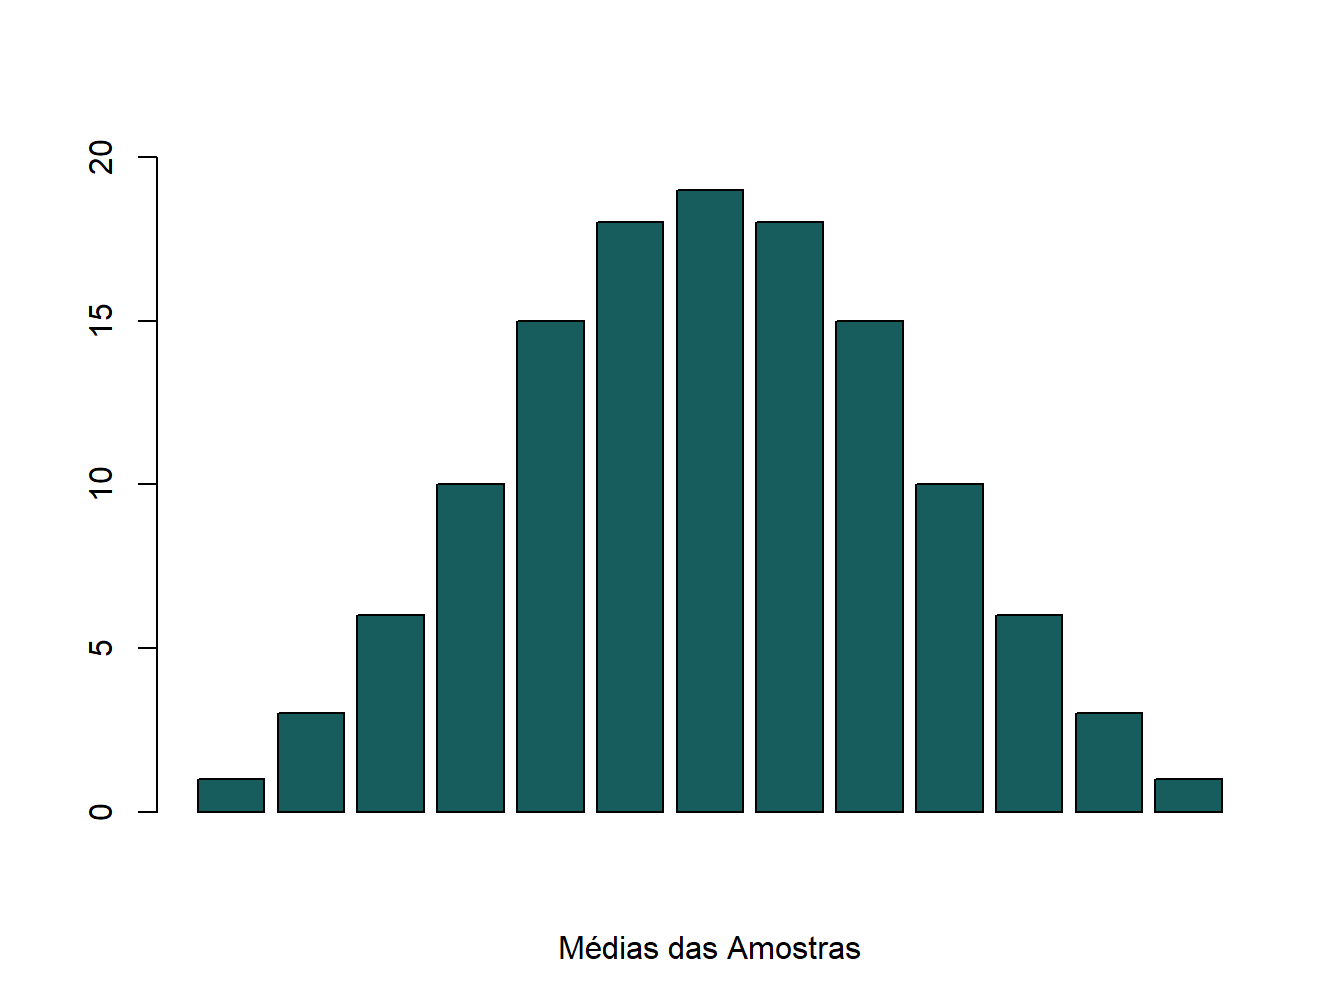
\includegraphics[width=0.8\linewidth]{bookdown-demo_files/figure-latex/DA4-1} 

}

\caption{Distribuição das médias das amostras de três elementos}\label{fig:DA4}
\end{figure}

Esse gráfico é muito semelhante ao gráfico da distribuição normal. Tem
um formato de sino, é simétrico, etc.

Outro fato interessante é que a média das médias amostrais é igual a 10
(parâmetro da média da população).

Além disso, supondo amostras com 03 elementos, com reposição. Será
possível estabelecer 125 possíveis resultados. A média desses resultados
será 10,00. O desvio padrão será 0,8185.

Considerando a distribuição Normal, se temos a média e o desvio padrão,
podemos utilizar a regra empírica 68\%, 95\%, 99,7\% para calcular
probabilidades do relacionamento entre a média da amostra e a média da
população.

\section{Aplicação prática}\label{aplicacao-pratica}

Vamos utilizar um exemplo real. No pacote chamado
\emph{TeachingSampling} tem uma base de dados com 2.396 linhas chamada
\textbf{Lucy}. O que queremos é extrair amostras aleatórias desse banco
de dados de diversos tamanhos e calcular o valor de \emph{Income}
(renda) médio.

\begin{Shaded}
\begin{Highlighting}[]
\KeywordTok{library}\NormalTok{(TeachingSampling)}
\KeywordTok{data}\NormalTok{(Lucy)}
\KeywordTok{dim}\NormalTok{(Lucy)}
\end{Highlighting}
\end{Shaded}

\begin{verbatim}
## [1] 2396    8
\end{verbatim}

Vamos extrair uma Amostra Aleatória Simples (AAS) desse banco de dados.
A amostra que vamos extrair será de tamanho igual a 400.

A função para fazer isso no R é \textbf{S.WR(N,m)}.Esse nome vem de:
\textbf{S}ampling \textbf{W}ith \textbf{R}eplacement (\textbf{N}=Tamanho
da população,\textbf{m}=Tamanho da Amostra)

\begin{Shaded}
\begin{Highlighting}[]
\NormalTok{N <-}\StringTok{ }\KeywordTok{dim}\NormalTok{(Lucy)[}\DecValTok{1}\NormalTok{]}
\NormalTok{m <-}\StringTok{ }\DecValTok{400}
\NormalTok{sam<-}\KeywordTok{S.WR}\NormalTok{(N,m)}
\NormalTok{data <-}\StringTok{ }\NormalTok{Lucy[sam,]}
\KeywordTok{dim}\NormalTok{(data)}
\end{Highlighting}
\end{Shaded}

\begin{verbatim}
## [1] 400   8
\end{verbatim}

\begin{Shaded}
\begin{Highlighting}[]
\KeywordTok{mean}\NormalTok{(Lucy}\OperatorTok{$}\NormalTok{Income)}
\end{Highlighting}
\end{Shaded}

\begin{verbatim}
## [1] 432.0605
\end{verbatim}

\begin{Shaded}
\begin{Highlighting}[]
\KeywordTok{mean}\NormalTok{(data}\OperatorTok{$}\NormalTok{Income)}
\end{Highlighting}
\end{Shaded}

\begin{verbatim}
## [1] 426.01
\end{verbatim}

A média da amostra não ficou próxima da média da população? E se
extrairmos outra amostra? \emph{Recomendo fortemente que você faça
isso}. O valor da amostra fica algo entorno do verdadeiro valor da
população, não? Isso porque os valores seguem uma distribuição Normal. O
que quero dizer com isso? Que as amostras não são extraidas para acertar
na mosca, mas sim para chegar bem perto do verdadeiro valor
populacional. Podemos então pensar em um intervalo em 95\% das vezes o
verdadeiro valor estará incluido. Esse é o tema do proximo capítulo.

Desse modo, podemos errar para mais ou para menos. A média da amostra
poder ser um pouco maior ou um pouco menor qie a média da população. Se
extrairmos muitas amostras, cad auma terá um média, mas espéramos que
elas difiram umas das outras e da média populacional por chance
aleatória.

\section{Exercício}\label{exercicio}

\begin{enumerate}
\def\labelenumi{\arabic{enumi}.}
\tightlist
\item
  Gerar uma população de tamanho 100.000 com média igual a 100 e desvio
  padrão igual a 20
\item
  Gerar uma amostra de tamanho 100
\item
  Calcular a média da população
\item
  Calcular a média da amostra
\item
  Ver a diferença entre a média da amostra e a média da população
\item
  repetir os passos 2 a 6 pelo menos cinco vezes
\end{enumerate}

\begin{Shaded}
\begin{Highlighting}[]
\CommentTok{# Definindo o tamanho da população e da amostra }
\NormalTok{N <-}\StringTok{ }\DecValTok{100000}
\NormalTok{m <-}\StringTok{ }\DecValTok{100}
\CommentTok{# Gerando uma conjunto de dados (Populacao)}
\NormalTok{Populacao<-}\StringTok{ }\KeywordTok{data.frame}\NormalTok{(}\KeywordTok{rnorm}\NormalTok{(N, }\DecValTok{100}\NormalTok{, }\DecValTok{20}\NormalTok{))}
\CommentTok{# Gerando uma amostra}
\NormalTok{sam<-}\KeywordTok{S.WR}\NormalTok{(N,m)}
\NormalTok{amostra <-}\StringTok{ }\KeywordTok{data.frame}\NormalTok{(Populacao[sam,])}
\CommentTok{# Comparando a distribuicao da amostra com a da populacao}
\KeywordTok{summary}\NormalTok{(amostra)}
\end{Highlighting}
\end{Shaded}

\begin{verbatim}
##  Populacao.sam...
##  Min.   : 53.20  
##  1st Qu.: 87.68  
##  Median : 99.03  
##  Mean   : 99.76  
##  3rd Qu.:113.68  
##  Max.   :149.88
\end{verbatim}

\begin{Shaded}
\begin{Highlighting}[]
\KeywordTok{summary}\NormalTok{(Populacao)}
\end{Highlighting}
\end{Shaded}

\begin{verbatim}
##  rnorm.N..100..20.
##  Min.   : 11.31   
##  1st Qu.: 86.56   
##  Median :100.00   
##  Mean   :100.02   
##  3rd Qu.:113.50   
##  Max.   :193.62
\end{verbatim}

Mais aplicações da relação da média da amostra com a média da população
pode ser \href{https://stevendutt.shinyapps.io/distamostral/}{encontrada
aqui}

\chapter{Intervalos de confiança}\label{intervalos-de-confianca}

Um intervalo de confiança (IC) é um intervalo estimado de um parâmetro
de interesse de uma população. Em vez de estimar o parâmetro por um
único valor, é dado um intervalo de estimativas prováveis.

Uma inferência sobre um parâmetro populacional deve fornecer não somente
uma estimativa por ponto (como a média), mas também indicar o quão
próximo a estimativa é provavel de estar do valor do parâmetro
\citet{Agresti}

A informação

\chapter{Teste de Hipóteses}\label{teste-de-hipoteses}

We describe our methods in this chapter.

\begin{Shaded}
\begin{Highlighting}[]
\KeywordTok{data}\NormalTok{(mtcars)}
\KeywordTok{library}\NormalTok{(nortest, }\DataTypeTok{pos=}\DecValTok{14}\NormalTok{)}
\KeywordTok{with}\NormalTok{(mtcars, }\KeywordTok{shapiro.test}\NormalTok{(mpg))}
\end{Highlighting}
\end{Shaded}

\chapter{Applications}\label{applications}

Some \emph{significant} applications are demonstrated in this chapter.

\section{Example one}\label{example-one}

\section{Example two}\label{example-two}

\chapter{Regressão Linear}\label{regressao-linear}

Vamos escrever um livro incrível

You can write citations, too. For example, we are using the
\textbf{bookdown} package \citep{R-bookdown} in this sample book, which
was built on top of R Markdown and \textbf{knitr} \citep{xie2015}.

\bibliography{packages,book}


\end{document}
